%%%%%%%%%%%%%%%%%%%%%%%%
%%%%%%%%% Préambule %%%%%%%%%
%%%%%%%%%%%%%%%%%%%%%%%%
\documentclass[a4paper,12pt]{article}
\usepackage{etex}

%%%%%Langue%%%%%

%%\usepackage[utf8]{inputenc}

\usepackage[T1]{fontenc}
\usepackage{babel} 
%%%%Police%%%%

%% MATHS BELLES : \usepackage{mathpazo}
%% TIMES NEW ROMAN :
\usepackage{stmaryrd}
\usepackage{newtxtext, newtxmath}
%%%%%Packages%%%%%

\usepackage[dvipsnames]{xcolor}

\usepackage{afterpage,amsfonts,amsmath,amssymb,amsthm,array,cancel,caption,comment,diagbox,dsfont,enumitem,fancybox,fancyhdr,float, framed,graphics,graphicx,hhline,import,latexsym,lscape,mathabx,multicol,multirow,pdfpages, setspace,subcaption,systeme,tikz,url,xcolor,mdframed}

\usepackage[left=2.5cm, right=2.5cm, top=2.5cm, bottom=2.5cm]{geometry}
\onehalfspacing
\usepackage[french,boxruled]{algorithm2e}
\usepackage[colorlinks=true]{hyperref} 
\usepackage[all]{xy}
\usepackage{dashundergaps}
\usepackage{pgfplots}
\usepackage{pdfpages}
\pgfplotsset{compat=1.18, width=10cm}
\dashundergapssetup{gap-extend-minimum=20pt,gap-extend-percent=20, gap-numbers=false,gap-format=dot,gap-widen=true,teacher-gap-format=dot}

\setlength{\columnsep}{0cm}

\usetikzlibrary{shapes.misc}
\newcommand{\mytimes}{ \tikz[baseline=-.55ex] \node [inner sep=0pt,cross out,draw,line width=1.5pt,minimum size=0.75ex] (a) {};}

\usepackage{tcolorbox}
\tcbuselibrary{theorems}

%%%%Couleurs%%%%

%Version en ligne

\definecolor{t2_red}{RGB}{210,12,70}
\definecolor{t2_blue}{RGB}{12,128,210}
\definecolor{t2_gold}{RGB}{210,180,12}
\definecolor{wooclap_blue}{RGB}{108,151,243}
\definecolor{t2}{RGB}{144,93,146}

%Version Imprimable

%\definecolor{t2_red}{RGB}{0,0,0}
%\definecolor{t2_blue}{RGB}{0,0,0}
%\definecolor{t2_gold}{RGB}{0,0,0}
%\definecolor{wooclap_blue}{RGB}{0,0,0}
%\definecolor{t2}{RGB}{0,0,0}

\hypersetup{urlcolor=t2_red,linkcolor=t2_red,citecolor=t2_red,colorlinks=true}


%%%%%Environnements%%%%%

\newtcbtheorem[number within=section]{defi}{Définition\,}{colback=t2_red!0,colframe=t2_blue,fonttitle=\bfseries}{df}

\newtcbtheorem[number within=section]{prop}{Proposition\,}{colback=t2_red!0,colframe=t2_red,fonttitle=\bfseries}{prop}

\newtcbtheorem[number within=section]{cor}{Corollaire\,}{colback=t2_red!0,colframe=t2_red,fonttitle=\bfseries}{cr}

\newtcbtheorem[number within=section]{theo}{Théorème\,}{colback=t2_red!0,colframe=t2_gold,fonttitle=\bfseries}{th}

\theoremstyle{definition}
%\newtheorem{conv}{Convention}
\newtheorem*{defin}{Définition}
\newtheorem*{ex}{Exemple}
\newtheorem*{exo}{Exercice}
\newtheorem*{corr}{Correction}
\newtheorem*{rap}{Rappel}
\newtheorem*{rem}{Remark}
\newtheorem*{que}{Question}
\newtheorem*{rems}{Remarques}
\theoremstyle{plain}
\newtheorem*{conj}{Conjecture}
\newtheorem*{demo}{Démonstration}
%\newtheorem{cor}{Corollaire}
%\newtheorem{princ}{Principe}
\newtheorem*{lem}{Lemme}
%\newtheorem{prop}{Proposition}
%\newtheorem{theo}{Théorème}
%\newtheorem*{theo_non_numero}{Théorème}

%\declaretheorem[name=Proposition,sibling=prop]{proprep}

%%%%%Macros%%%%%

%%Ensembles%classiques%%

\def\N{\mathbb{N}}%entiers naturels
\def\Z{\mathbb{Z}}%entiers relatifs
\def\Q{\mathbb{Q}}%rationnels
\def\R{\mathbb{R}}%réels
\def\C{\mathbb{C}}%complexes

%%Algèbre%linéaire%%

\def\codim{\mathrm{codim}}%codimension
\def\ker{\mathrm{ker}\,}%noyau
\def\coker{\mathrm{coker}\,}%conoyau
\def\im{\mathrm{im}\,}%image
\def\id{\mathrm{id}}%application identité
\newcommand\scal[2]{\langle #1,#2\rangle}%produit scalaire

%%Géométrie%différentielle%%

\def\grad{\mathrm{grad}}%gradient
\def\ind{\mathrm{ind}\,}%indice
\def\modu{\mathcal{M}}%espace de modules
\def\moduc{\overline{\mathcal{M}}}%espace de modules compactifié
\def\moducbullet{\overline{\mathcal{M}_\bullet}}%espace de modules avec un point marqué compactifié
\def\ev{\mathrm{ev}}%applications évaluations dans la base
\def\Ev{\mathrm{Ev}}%applications évaluations dans l'espace total
\def\lacet{\ell}%lacet de Morse
\def\lacets{\mathcal{L}}%lacets de Morse
\newcommand\ro{roulement}%roulement-crocodile
\newcommand\Star{{S_\star}}%ensemble du point étoilé et des augmentations
\newcommand\fibrEv{\underset{\Ev}{\boxtimes}}%produit fibré des évaluations dans l'espace total
\newcommand\fibrev{\underset{\mathrm{ev}}{\boxtimes}}%produit fibré des évaluations dans la base
\newcommand\moducmix[1]{\overline{\modu^{#1}}}%espace de modules mixtes
\newcommand\moducmixbul[1]{\overline{\modu^{#1}_\bullet}}%espace de modules à rebonds
\newcommand\moducprime{\overline{\mathcal{M}'}}%espace de modules pour un second jeu de données
\newcommand\rg{\mathfrak{r}}
\newcommand\qg{\mathfrak{q}}
\newcommand\Loop{\mathcal{L}}
\newcommand\push{\Phi}
\newcommand\drum{drumroll}

%%%%%Commandes%%%%%

\def\;{\,\,;\,\,}%point virgule espacé

\def\tq{\,\,\mathrm{t.q.}\,\,}%tel que

\def\iff{\Longleftrightarrow}%équivaut à, la commande initiale ne marche pas

\def\implies{\Longrightarrow}%implique, la commande initiale ne marche pas

\newcommand\fonction[5]{#1:
	\begin{array}{ccc}
		#2&\longrightarrow &#3\\
		#4&\longmapsto &#5
\end{array}}%fonction avec ensembles de départ, d'arrivée et transformation

\newcommand\fonctionbira[5]{#1:
	\begin{array}{ccc}
		#2&\dashrightarrow &#3\\
		#4&\longmapsto &#5
\end{array}}

\newcommand\fonctionnonnommee[4]{\begin{array}{ccc}
		#1 &\longrightarrow& #2\\
		#3 &\longmapsto & #4
\end{array}}%fonction avec ensembles de départ, d'arrivée et transformation, sans nom

%%%%Tables%%%%
\usepackage{adjustbox}
\usepackage{booktabs}

%%%%%Bibliographie%%%%%

\bibliographystyle{alpha-en}

%%%%%Style%%%%%

\pagestyle{empty}
\pagestyle{fancy}

\setlength{\headheight}{16pt}
\usepackage{listings}

\definecolor{darkWhite}{rgb}{0.94,0.94,0.94}

\lstset{
	aboveskip=3mm,
	belowskip=-2mm,
	backgroundcolor=\color{darkWhite},
	basicstyle=\footnotesize,
	breakatwhitespace=false,
	breaklines=true,
	captionpos=b,
	commentstyle=\color{red},
	deletekeywords={...},
	escapeinside={\%*}{*)},
	extendedchars=true,
	framexleftmargin=16pt,
	framextopmargin=3pt,
	framexbottommargin=6pt,
	frame=tb,
	keepspaces=true,
	keywordstyle=\color{blue},
	language=C,
	literate=
	{²}{{\textsuperscript{2}}}1
	{⁴}{{\textsuperscript{4}}}1
	{⁶}{{\textsuperscript{6}}}1
	{⁸}{{\textsuperscript{8}}}1
	{€}{{\euro{}}}1
	{é}{{\'e}}1
	{è}{{\`{e}}}1
	{ê}{{\^{e}}}1
	{ë}{{\¨{e}}}1
	{É}{{\'{E}}}1
	{Ê}{{\^{E}}}1
	{û}{{\^{u}}}1
	{ù}{{\`{u}}}1
	{â}{{\^{a}}}1
	{à}{{\`{a}}}1
	{á}{{\'{a}}}1
	{ã}{{\~{a}}}1
	{Á}{{\'{A}}}1
	{Â}{{\^{A}}}1
	{Ã}{{\~{A}}}1
	{ç}{{\c{c}}}1
	{Ç}{{\c{C}}}1
	{õ}{{\~{o}}}1
	{ó}{{\'{o}}}1
	{ô}{{\^{o}}}1
	{Õ}{{\~{O}}}1
	{Ó}{{\'{O}}}1
	{Ô}{{\^{O}}}1
	{î}{{\^{i}}}1
	{Î}{{\^{I}}}1
	{í}{{\'{i}}}1
	{Í}{{\~{Í}}}1,
	morekeywords={*,...},
	numbers=left,
	numbersep=10pt,
	numberstyle=\tiny\color{black},
	rulecolor=\color{black},
	showspaces=false,
	showstringspaces=false,
	showtabs=false,
	stepnumber=1,
	stringstyle=\color{gray},
	tabsize=4,
	title=\lstname,
}

\title{Evaluation Of Spectral Clustering methods.}
\author{Malik Hacini}
\begin{document}
	\maketitle
	\tableofcontents
	\section{Introduction}
	This document presents the methods, experiments and results achieved for spectral clustering on synthetic and real world datasets. All of the project was written in Python. You will find the code referenced in this presentation in the "src" folder of the project. For more information on spectral clustering, refer to PH.
	\section{Code architecture}
	The code for this project is divided into 2 main Python files :
	\begin{itemize}
		\item graphs.py
		\item spectralclustering.py
	\end{itemize}
	The goal of the structure is to be versatile: to perform a new experiment, you do not need to modify the code, as the different parameters give a lot of flexibility.
	\subsection{graphs.py}
	This file contains everything needed to the construction of a graph from a dataset. There is a "Graph" Python class meant to create a graph based on a list of data points. 
	With class attributes and methods, you can then access all of the spectral clustering related objects of the graph : adjacency matrix and laplacians (with all kinds implemented).
	
	One key feature of these graphs is the similarity function used. A "Similarity" Python class exists for this purpose. However, in most cases , we use the gaussian kernel similarity function, hence it is the default one in our implementation.
	
	Lastly, there is a symmetrizing method parameter. It is the method used for symmetrizing the adjacency matrix in the case of classical spectral clustering. The choices are "mean, or, and". Please refer to the source code for more details.
	Overall, this file is all you need to construct a graph based on your dataset.
	\begin{ex}
		Consider a dataset "data" where we want to build a 10-nn graph G using the gaussian kernel of standard deviation $\frac{1}{2}$ and symmetrizing the adjacency matrix by the 'mean' method, the call would be :
		\begin{lstlisting}
			G=Graph(data,10,'knn','mean',1/2)
		\end{lstlisting}
		We can then easily access the graph adjacency matrix and laplacians using the Graph class attributes and methods.
	\end{ex}
	\subsection{spectralclustering.py}
	This file contains everything needed to perform spectral clustering on a dataset, it's main function being simply called "spectral clustering".
	Understanding this functions's parameters is the only real thing you need to conduct experiments using spectral clustering. Here is the docstring associated with it :
	\begin{lstlisting}
		def spectral_clustering(data,k_neighbors,n_eig,laplacian,g_method='g_knn',sym_method='mean',sigma=None,use_minibatch=False,eigen_only=False,clusters_fixed=False,return_matrix=False,labels_given=np.array([None])):
		"""Performs spectral clustering on a dataset of n-dimensional points.
		Inputs :
		data (ndarray): The dataset, a 
		k_neighbors (int): Number of neighbors you want to connect in the case of a k-nn graph.
		n_eig (int): Number of eigenvectors to calculate. Used to compute the number of clusters
		laplacian (string) : The laplacian to use between [un_norm , sym , rw] 
		sym_method (string): The method used to symmetrize the graph matrix in the case of an asymmetric adjacency matrix.
		sigma (float): Standard deviation for the gaussian kernel.
		use_minibatch (bool) : Choice of the k-means algorithm. True might lead to better performance on large datasets. Default = False.
		eigen_only (bool) : If True, the function will only returns the eigenvalues and eigenvectors and not compute the full clustering. Default = False.
		clusters_fixed (int) : The number of clusters in your data. If unknown, leave by default and the eigengap heuristic will be used. Default = False.
		return_matrix (bool) : True <=> returns the adjacency matrix alongside the clustering results. Use if you want to visualize the graph. Default = False.
		labels_given (ndarray) : The correct labels of your data. If given, used to reorder the labels obtained by clustering. Leave empty if unknown. Default = False 

		Returns :
		vals (ndarray): the computed eigenvalues pf the graph laplacian.
		labels (ndarray) : labels of the points after spectral clustering, ordered in the same way as the dataset.
		matrix (ndarray) : the adjacency matrix of the graph
		"""
	\end{lstlisting}

	
\section{Spectral Clustering Experiments}
This section summarizes the experiments done.
\subsection{Basic Experiments}
To assert the good behavior of our algorithms, the first step was to conduct very basic experiments. We are going to use very simple toy datasets and focus on 2 important results : Clustering performance and Eigenvalues of laplacians.
\subsubsection{Circles and Moons}
The most basic spectral clustering example are the circles and moons dataset. These datasets fail to be clustered correctly by $k$-means, as the clusters do not lie in disjoint convex sets. However, spectral clustering is powerful enough to correctly cluster these datasets.
Due to the simplicity of the datasets, practically any choice of settings gives perfect performance.
\begin{figure}[H]
	\begin{subfigure}{.6\textwidth}
		\centering
		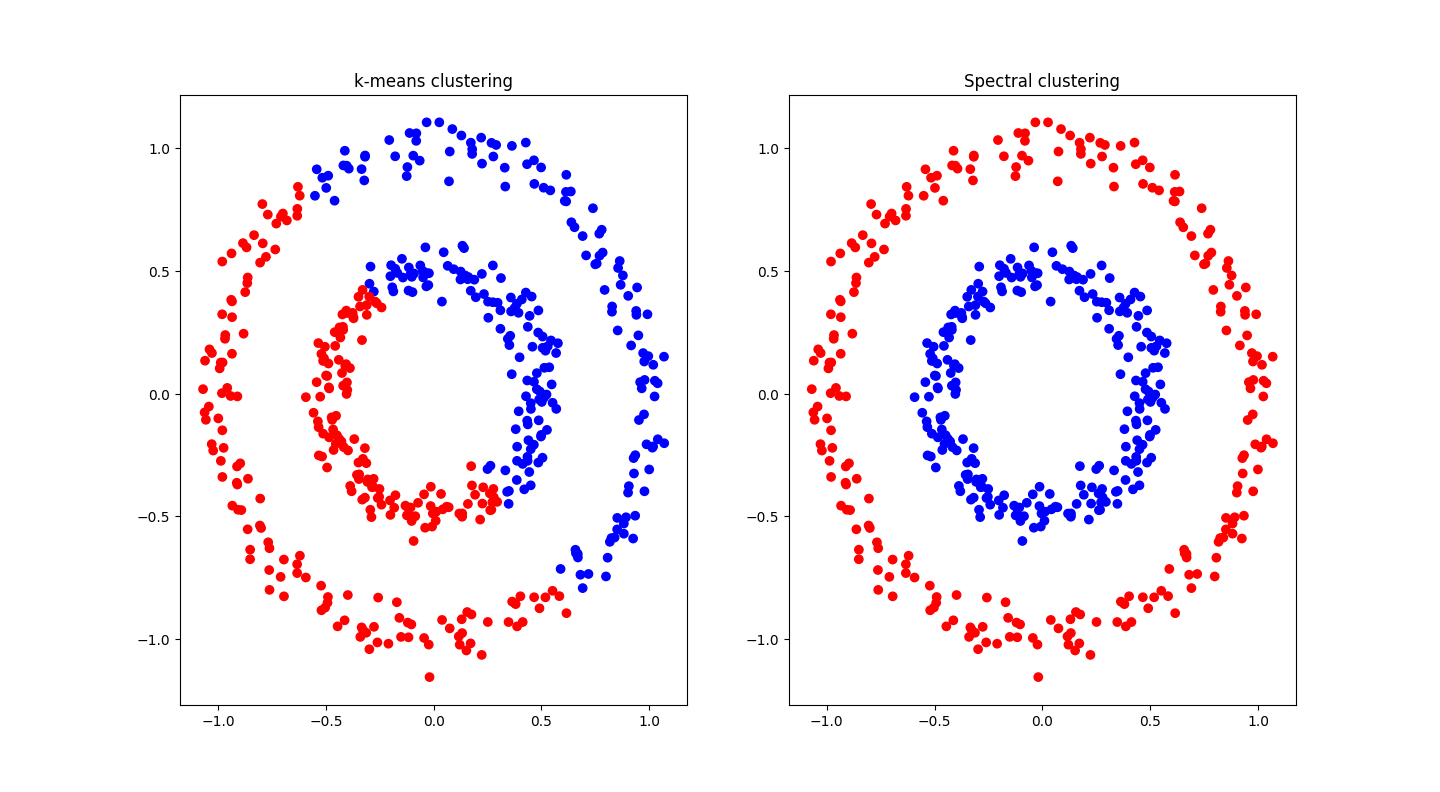
\includegraphics[width=0.9\linewidth]{figures/Fig1}
		\caption{Circles}
	\end{subfigure}
	\begin{subfigure}{.6\textwidth}
		\centering
		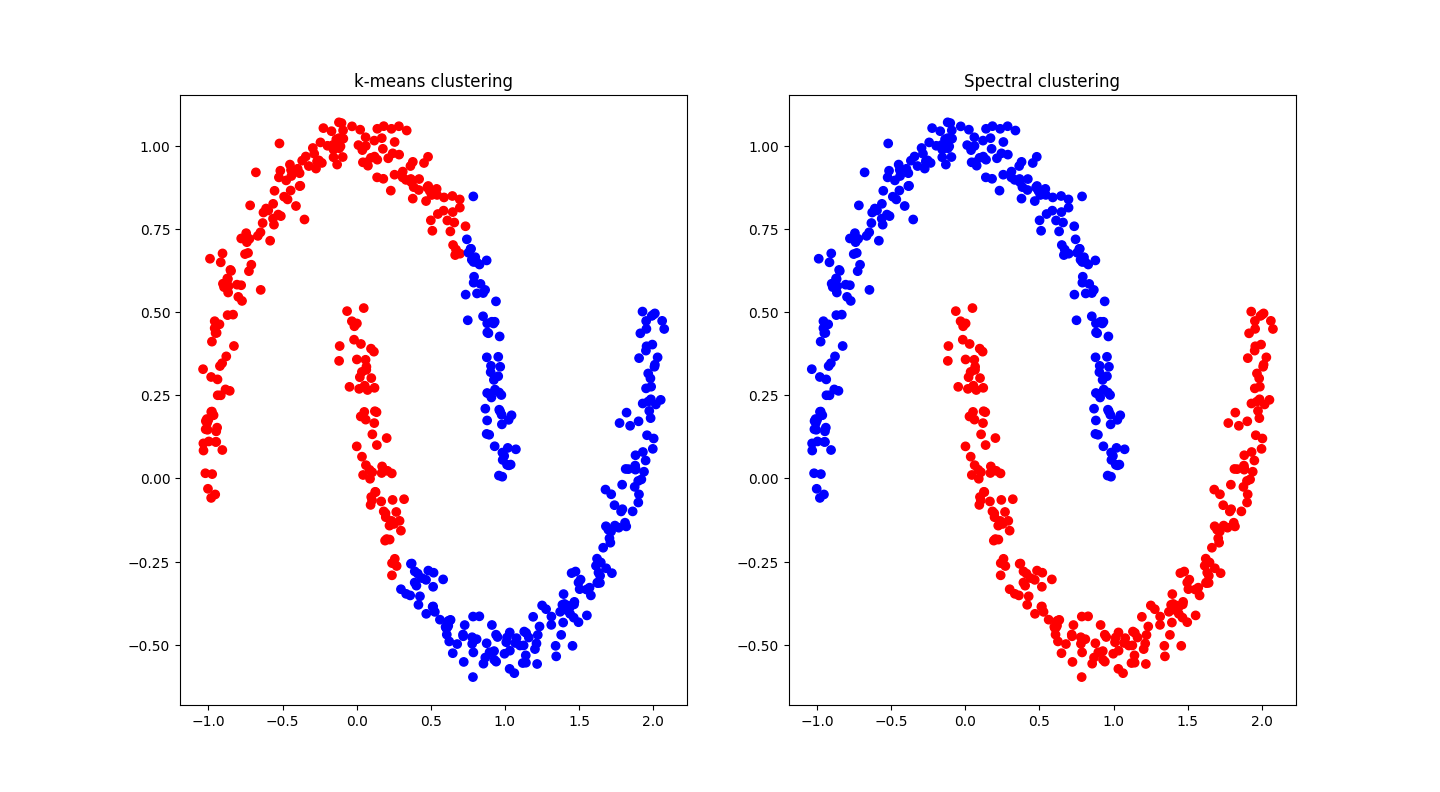
\includegraphics[width=0.9\linewidth]{figures/Fig2}
		\caption{Moons}
	\end{subfigure}
	\caption{Comparison between $k$-means and spectral clustering on toy datasets}
\end{figure}


In this experiment, we know the correct number of clusters because we can visualize the dataset, which isn't always the case for real datasets. To get a hint on the correct number of clusters, sectral clustering offers the eigengap heuristic. For most datasets, the quality of the eigengap will be different depending on the laplacian. However, in very simple cases like circles and moons, the $k$-nn graph is disconnected into the two clusters, which is the ideal theoretical case for the eigengap heuristic, thus every laplacian leads to a good eigengap :


\begin{figure}[H]
	\captionsetup{justification=centering}
	\centering
	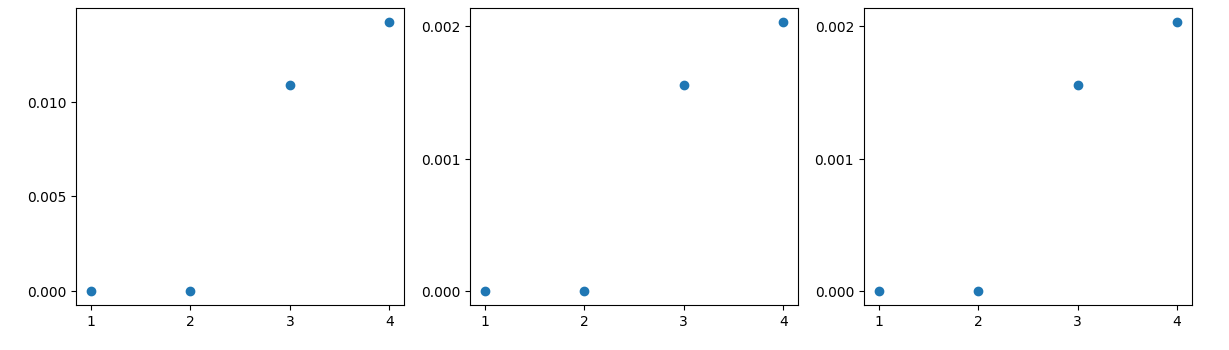
\includegraphics[width=1.1\linewidth]{figures/Fig_E1_circles}
	\caption{First eigenvalues of laplacians for the clustering of the circles dataset. \\ Left to right : $L$, $L_{sym}$, $L_{rw}$}
	\label{fig:fige1circles}
\end{figure}

Every laplacian has a gap in it's eigenvalues after 2 of them, meaning the graph contains exactly 2 connected components, thus 2 clusters.
In order to show the difference between each laplacian, we need more sophisticated datasets.

\subsubsection{Gaussian Mixture Models (GMMs)}
In the goal of doing qualitative comparison between different methods, using $2$-dimensional gauussian mixture datasets is a good starting point. 
\paragraph{Multivariate Normal Distribution} The multivariate normal distribution, also called "multivariate gaussian" is a generalization of the one-dimensional (univariate) normal distribution to higher dimensions. For any dimension $d$, it can be defined by it's PDF :
$$\fonctionnonnommee{\R^{d}}{\R_{>0}}{x}{\frac{1}{\sqrt{(2\pi)^2 \lvert \Sigma \rvert}} e^{-\frac{1}{2}(x-\mu) \Sigma^{-1} (x-\mu)^{t}}}$$
Where:
\begin{itemize}
	\item $\mu \in{R^d}$ is the mean of the distribution.
	\item $\Sigma$ is a $d$ by $d$ square symmetric positive semi-definite matrix called the covariance matrix, because when $x$ is treated as a random vector with each of it's coordinates $x_i$ being a random variable, $\sigma_{i,j}= Cov(x_{i},x_{j})$.
\end{itemize}
The multivariate gaussian distribution is centered at $\mu$ and has an ellipsoidal shape defined by $\Sigma$.
\begin{figure}[H]
	\centering
	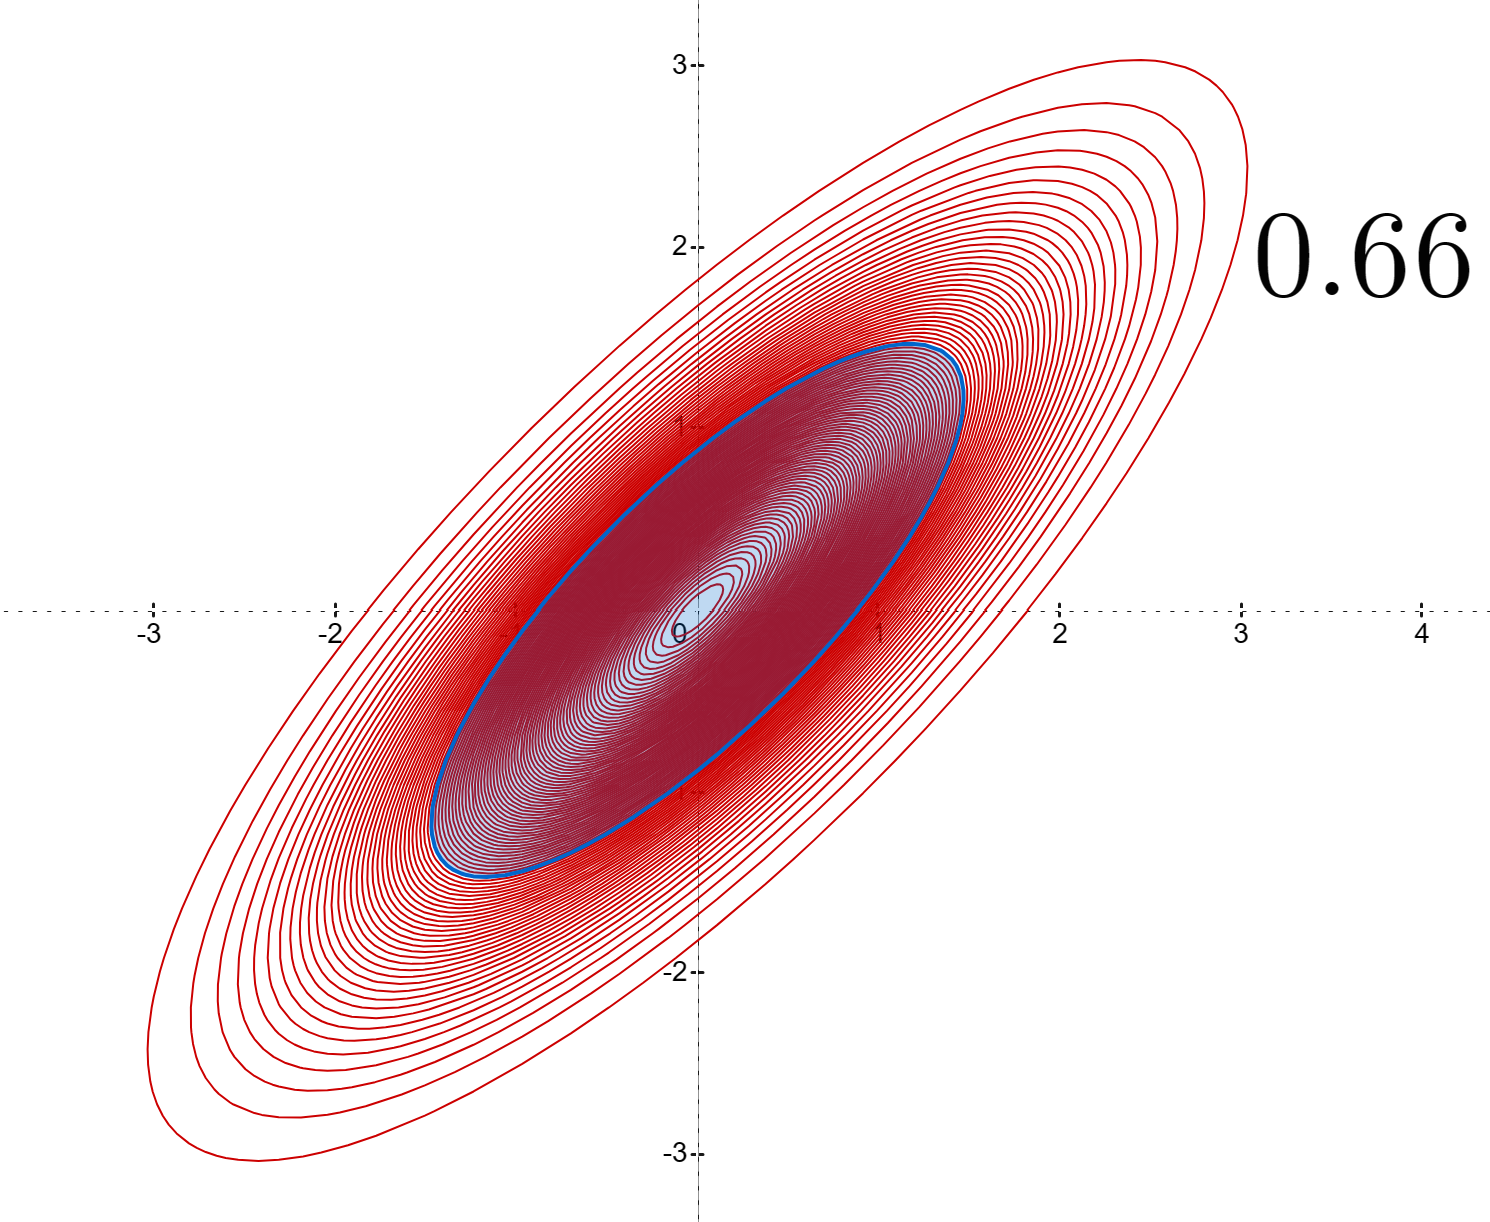
\includegraphics[width=0.4\linewidth]{figures/Binorm}
	\caption{Level sets of a bivariate normal distribution centered at the origin. The probability of a sample landing in the blue ellipse is $0.66$.}
	\label{fig:binorm}
\end{figure}

A linear combination of $d$-dimensional gaussians is called a gaussian mixture.
\begin{figure}[H]
	\centering
	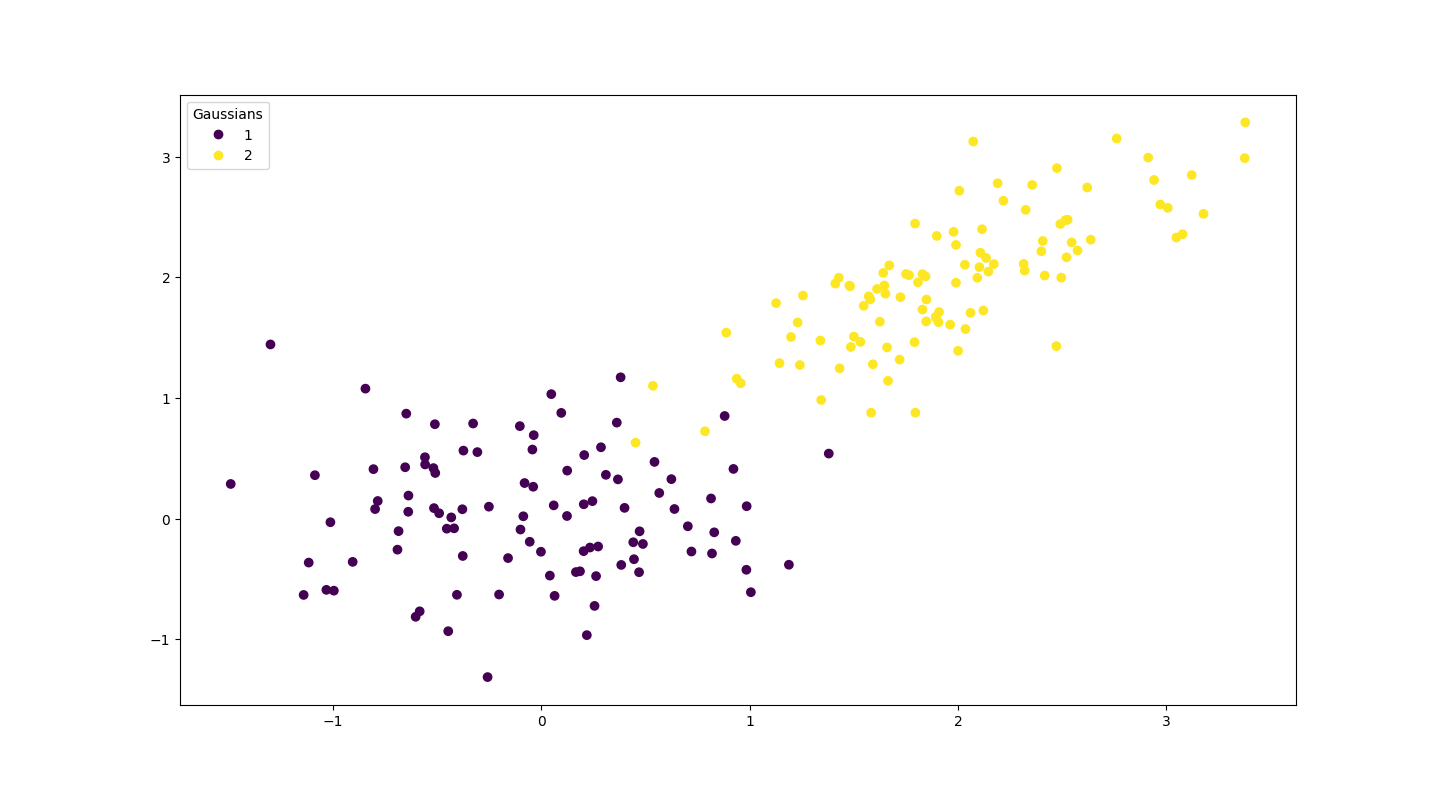
\includegraphics[width=0.6\linewidth]{figures/2gm}
	\caption{$200$ samples from a mixture of two 2-dimensional gaussians.}
	\label{fig:2gm}
\end{figure}
\begin{rem} 
	In practice, since gaussians PDF decay quickly when driving away from $\mu$, when the means are fairly spaced, the different gaussians do not really interact to form a diffrent PDF and the resulting mixture just looks like a superpostion of the respective gaussians. Thus, we do not perform the sampling with the actual PDF of the mixture, but uniformly choose between the different gaussians for each point.
\end{rem}
Gaussian mixtures form great toy datasets on which we can test and visualize our clustering, where a goal cluster is all of the points sampled from a particular gaussian.

\begin{figure}[H]
	\captionsetup{justification=centering}
	\begin{subfigure}{.6\textwidth}
		\centering
		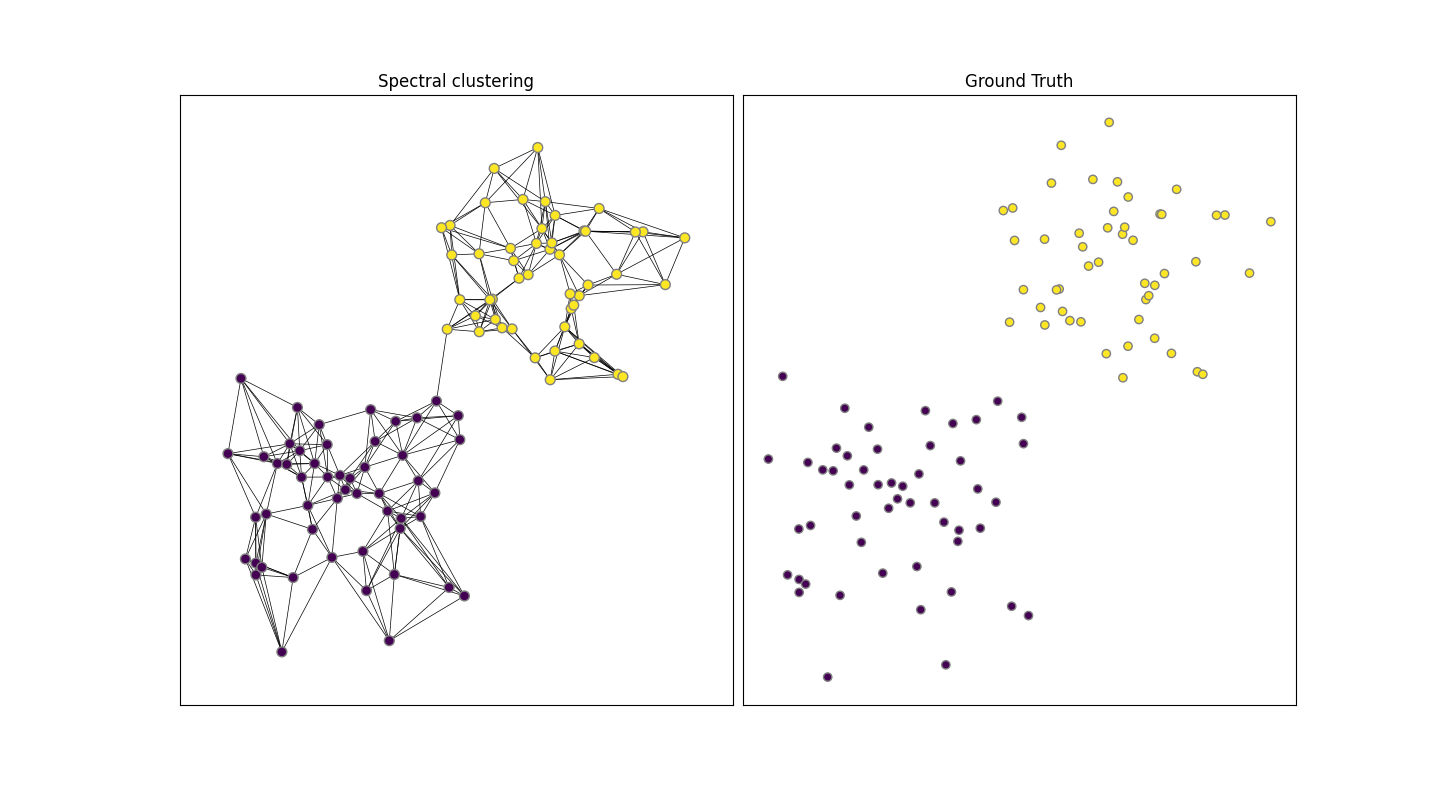
\includegraphics[width=0.9\linewidth]{figures/fig5_g1}
		\caption{Successful clustering}
	\end{subfigure}
	\begin{subfigure}{.6\textwidth}
		\centering
		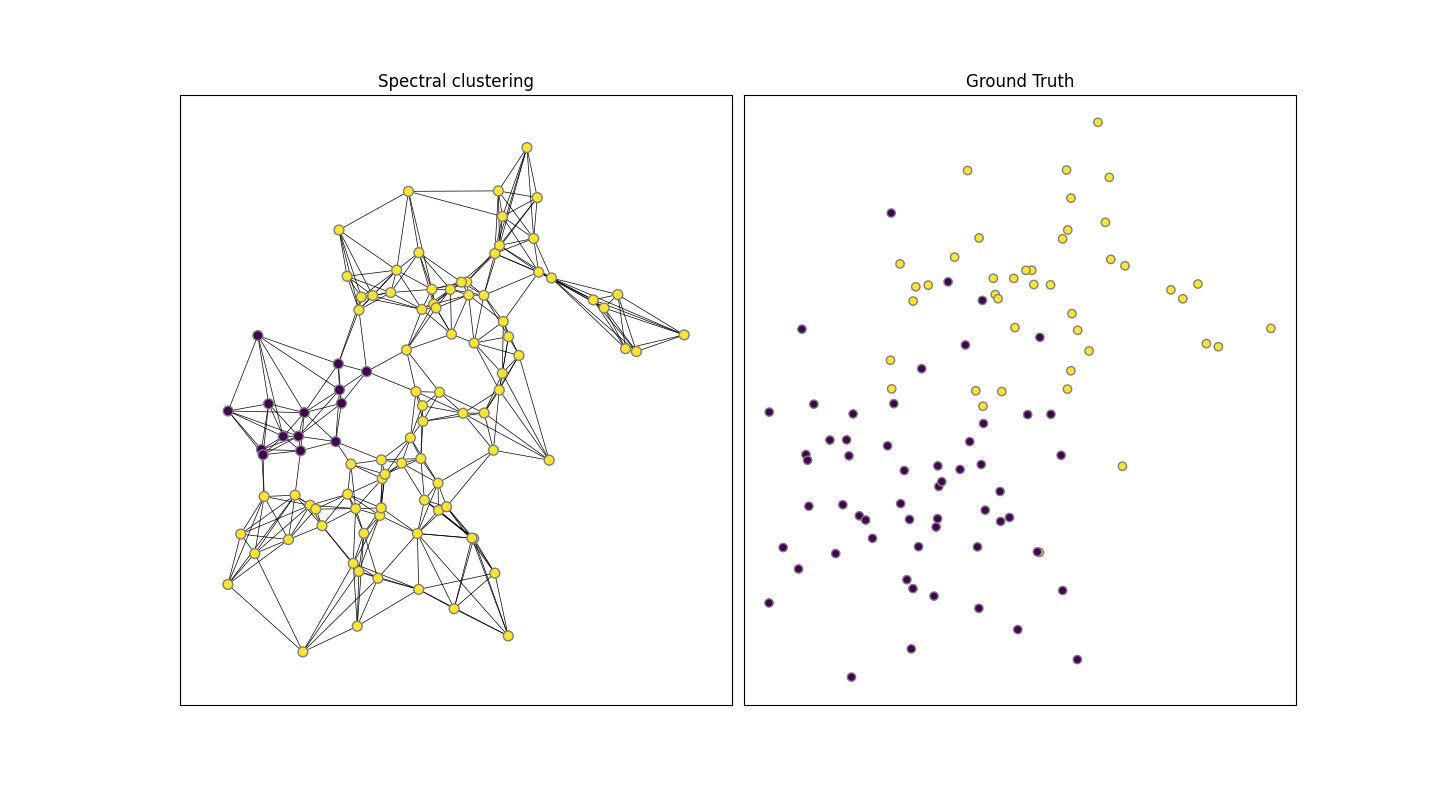
\includegraphics[width=0.9\linewidth]{figures/fig6_g2}
		\caption{Unsuccessful clustering}
	\end{subfigure}
	\caption{Visualization of spectral clustering and it's $k$-nn graph on a gaussian mixture. \\ Settings : $L_{rw}$, $k=6$, $\sigma=\frac{1}{3}$ (for gaussian kernel).}
\end{figure}
On figure (a) we see that the $k$-nn graph well encodes the cluster structure of the data. It is fully connected but there is only one link between clusters, which makes for great performance of SC using $L_{rw}$. \\ \\
On figure (b), the means of the two gaussians are closer apart, thus the clustering fails to partition the graph correctly due to the multiple links between the real clusters.
However, increasing $k$ creates stronger links inside of the clusters, leading to better performance : 
\begin{figure}[H] 
	\label{unsuc}
	\centering
	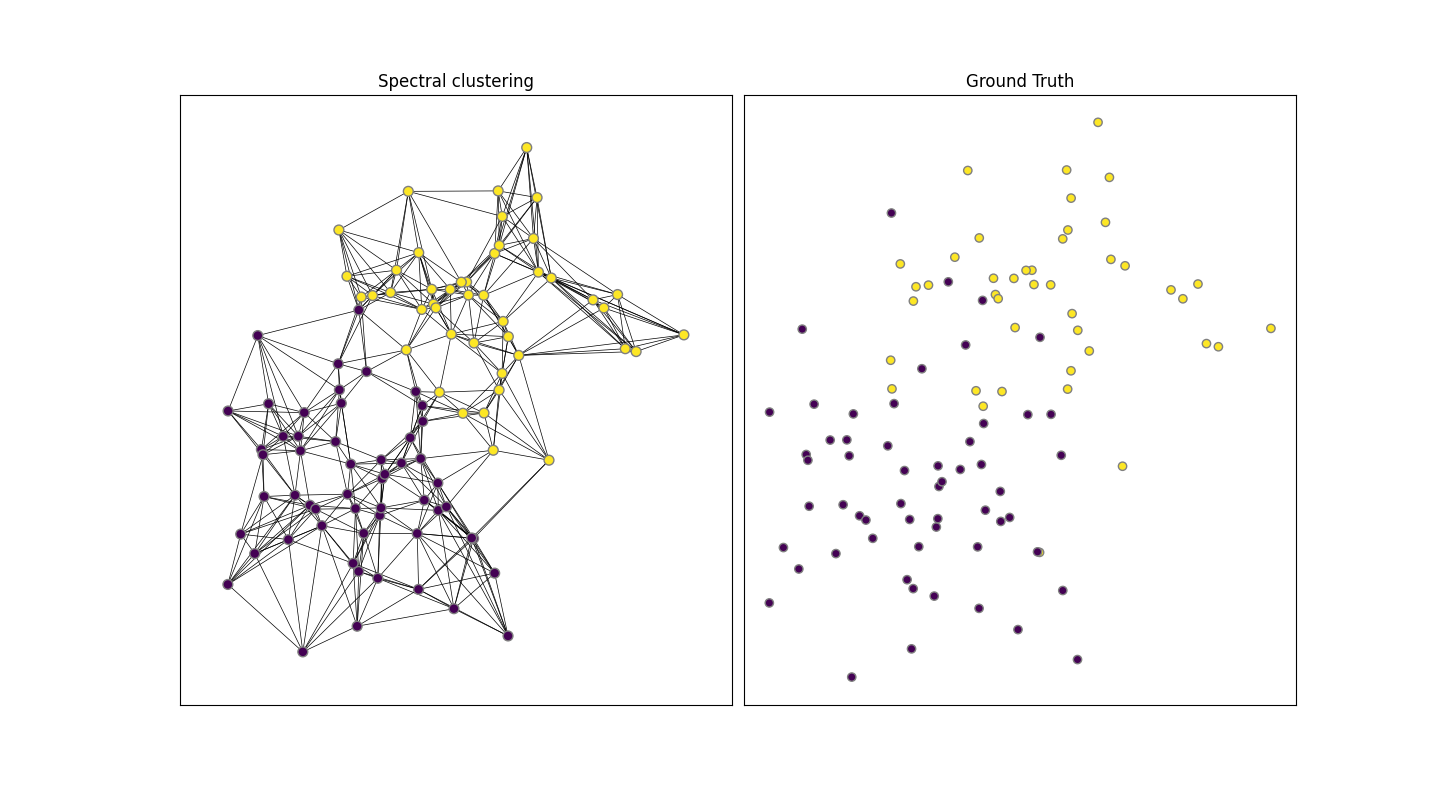
\includegraphics[width=0.6\linewidth]{figures/fig7_g3}
	\caption{The performance of the clustering is increased with $k=8$}
	\label{fig:fig7g3}
\end{figure}
By forcing the algorithm to form $2$ clusters, we get good performance. Again, what if we didn't know the true number of clusters ? In this case, the graph is fully connected, so does the eigengap really indicates $2$ clusters ? 

\begin{figure}[H]
	\captionsetup{justification=centering}
	\begin{subfigure}{.3\textwidth}
		\centering
		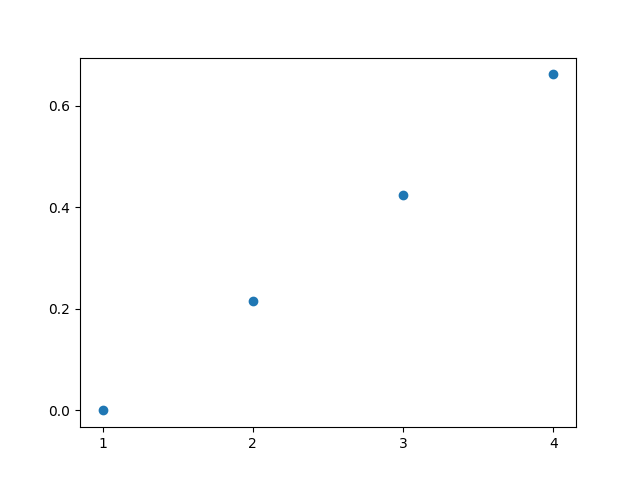
\includegraphics[width=1.1\linewidth]{figures/Fig_E4_L}
		\caption{$L$}
	\end{subfigure}
	\begin{subfigure}{.3\textwidth}
		\centering
		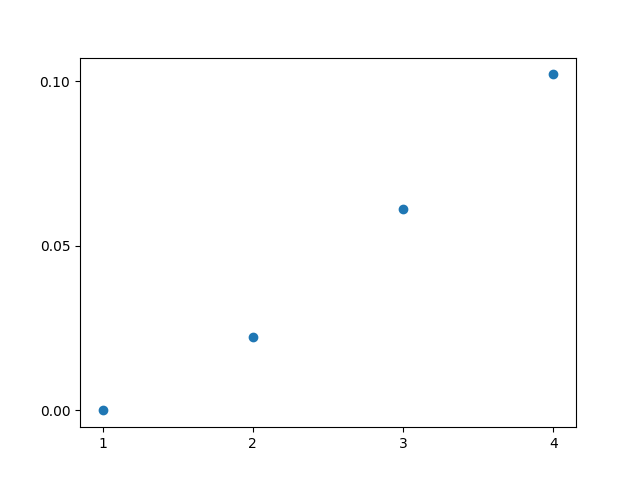
\includegraphics[width=1.1\linewidth]{figures/Fig_E5_L_sym}
		\caption{$L_{sym}$}
	\end{subfigure}
	\begin{subfigure}{.3\textwidth}
		\centering
		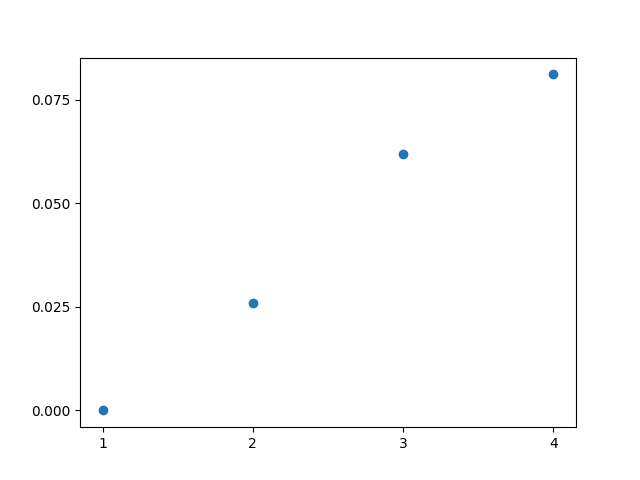
\includegraphics[width=1.1\linewidth]{figures/Fig_E6_L_rw}
		\caption{$L_{rw}$}
	\end{subfigure}
	\caption{First eigenvalues of laplacians for the graph of \ref{unsuc}.}
\end{figure}
These results clearly show that the connectivity of the graph has great impact of the quality of the eigengap. Both the spectra of $L$ and $L_{rw}$ give no valuable information and while $L_{sym}$ does have a "gap" after the second eigenvalue, it isn't clear enough to conclude on the true number of clusters.
In conclusion, while the eigengap can be a useful criteria in the case of well separated datasets, when the graph is strongly connected to better the performance on harder datasets, the eigengap becomes meaningles as noise is too big.
Thus, we conclude that to efficiently choose $k$, we need to connect the graph enough to ensure good performance, but not too much to the point where the eigengap is useless, otherwise we will be unable to know the correct number of clusters.
\subsection{Extensive study of the eigengap}
\subsubsection{Method}
$k$ is not the only parameter with an impact on the eigengap. In this section we investigate characteristics of synthetic $2$-d datasets to assess their impact on the eigengap. For this study, we also consider the generalized spectral clustering (GSC) framework proposed by \cite[Jonckheere et.al]{GSC}. In theory, this framework involves new parameters $(t,\gamma,\alpha)$ and two new laplacians $L_{G}$ and $L_{G_{rw}}$. In practice, we fix $(t,\gamma,\alpha)$=$(3,0.7,0.9)$ for every dataset. To simplify the study, we first consider the case of $2$ clusters. We investigate $3$ features of the datasets:
\begin{itemize}
	\item Geometry of clusters (shape and $D$-symmetry)
	\item $N$-symmetry
	\item Total number of points.
\end{itemize}
The big idea is to detect if clusters that "look alike" lead to better eigengaps. 
"Geometry of clusters" refers to the shape of the clusters. $2$ clusters are $N$-symmetric if they have the same number of points, and $D$-symmetric if they have the same (geometrical) density of points in the space they lie in.
To test these criteria, we generate multiple datasets and cluster them using every standard laplacian ($L$,$L_{sym}$,$L_{rw}$) and the generalized laplacians $L_G$ and $L_{G_{rw}}$. We make sure to separate these clusters well, to isolate the effect of our criteria on the eigengap. We are then able to choose $k$ efficiently as the datasets are on the easier side. The choice of $k$ is detailed in TOREF In practice, the standard laplacians return nearly identical results regarding performance of clustering and eigengap, thus we choose to only report $L_{rw}$ results and compare them to the generalized laplacians.
\subsubsection{Results}
\paragraph{Geometry of clusters.}
To correctly isolate the effect of the geometry of clusters, we build $N$-symmetric and $D$-symmeytric datasets. We start by a dataset with $2$ circular clusters to serve as reference.
We get the best results with $L_{G_{rw}}$.
\begin{figure}[H]
	\centering
	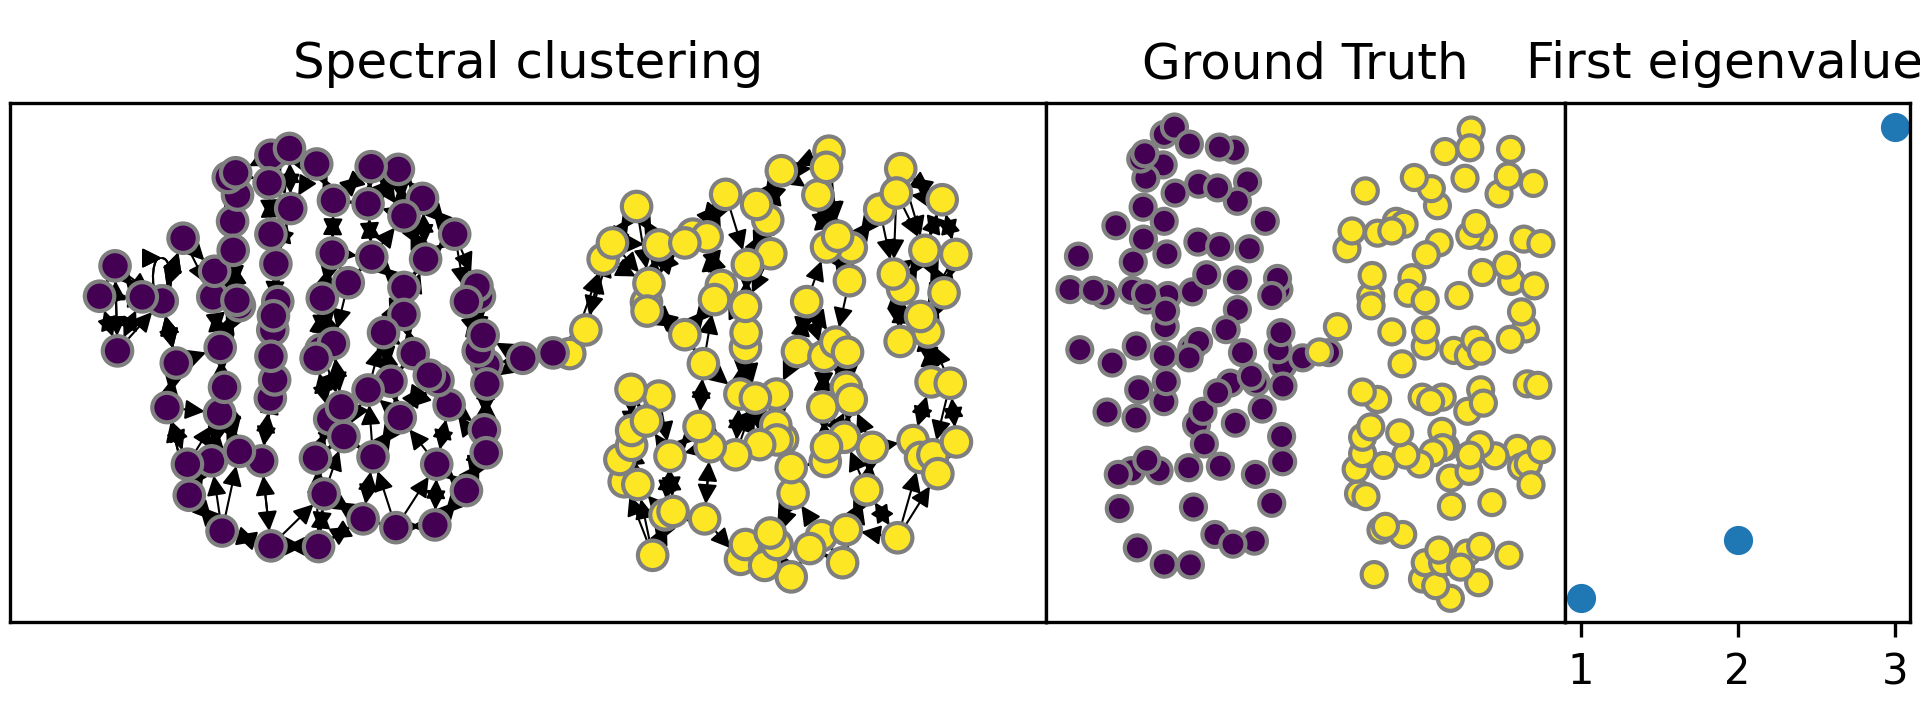
\includegraphics[width=0.6\linewidth]{figures/base_circles_g_rw}
	\label{fig:base_circles}
	\caption{$k$ = 4, $L_{G_{rw}}$. A great eigengap is observed.}
\end{figure}
As shown by the next experiment, changing the shape of one cluster doesn't change these results :
\begin{figure}[H]
	\centering
	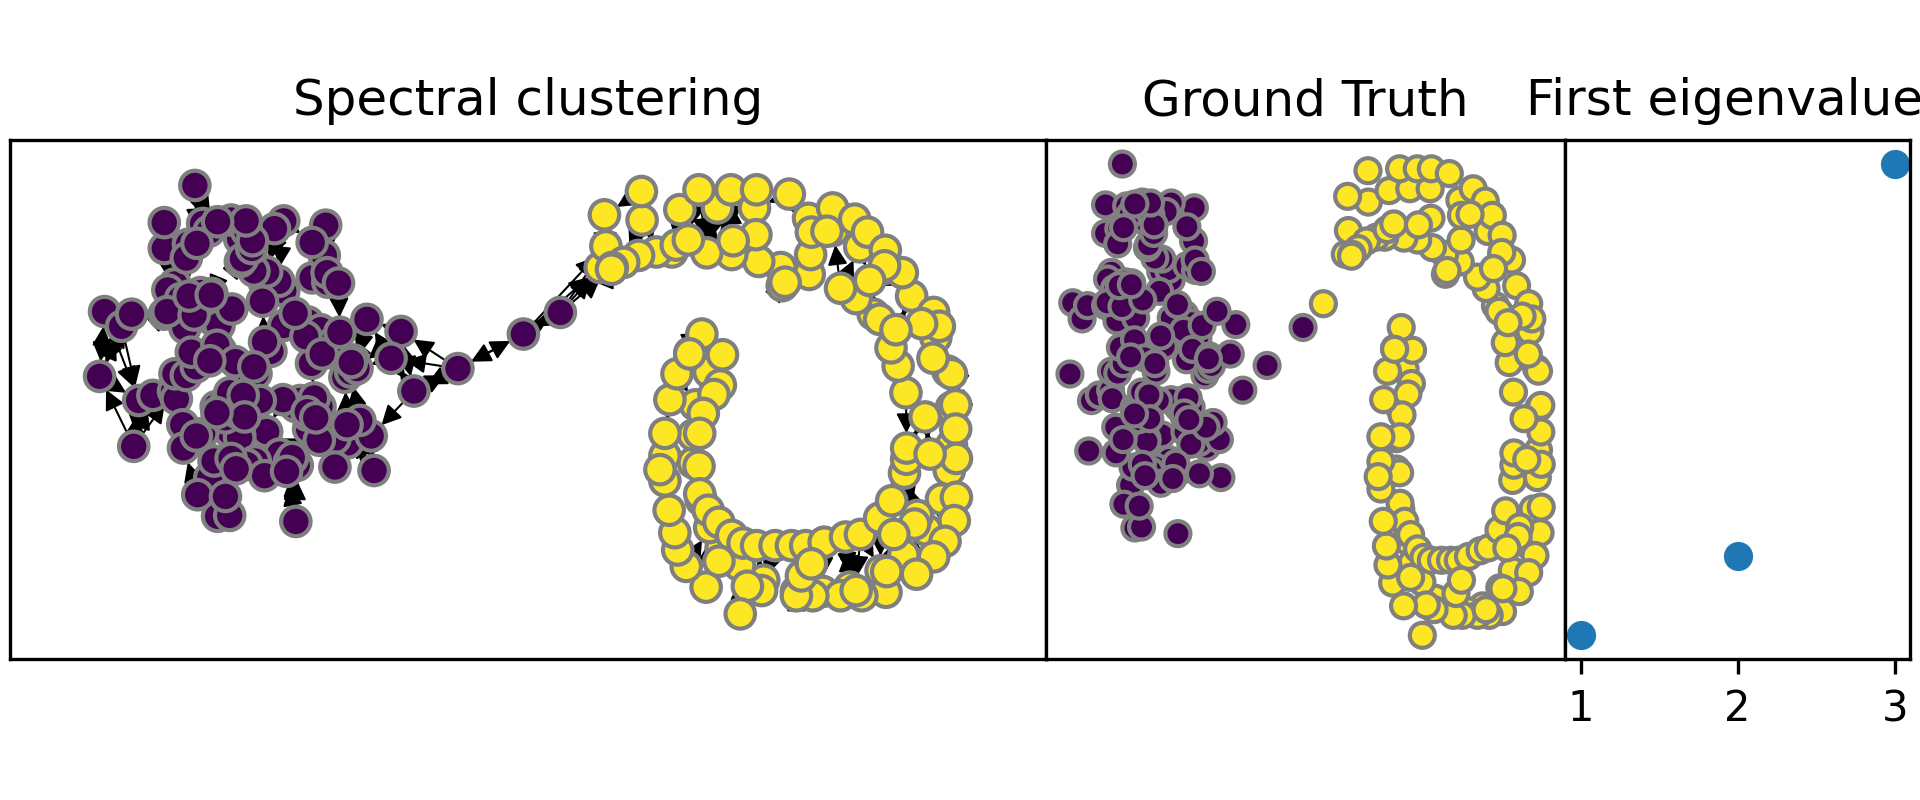
\includegraphics[width=0.6\linewidth]{figures/uneven_blobs_g_rw}
	\label{fig:uneven_blobs}
	\caption{$k$ = 4, $L_{G_{rw}}$. An eigengap of the same quality is observed.}
\end{figure}

Other experiments allow us to conclude that the shape of the clusters has no significant impact on the performance of the clustering and the quality of the eigengap.
These results were to be excpected : spectral clustering looks for the connected components of a $k$-nn graph. This graph does not contain the information of the shape of the clusters : in the adjacency matrix, a circular cluster will appear the same as an highly complex non-convex one. The underlying geometry of the subset of $\R^N$ a cluster belongs to is not taken into account when forming the graph, as only it's $k$- nearest neighbors are considered connected to him. This is an advantage spectral clustering has over $k$-means, which looks for convex clusters in $\R^N$. It is the main concept that makes up for the great performance of spectral clustering. \\
For the sake of simplicty and without loss of generality, we thus only consider circular clusters for our experiments on $N$-symmetry and $D$-symmetry.
\paragraph{$N$-symmetry}
To isolate the impact of $N$-symmetry, we consider datasets with a fixed number of points.

\subsection{UCI datasets}
Now that we know our algorithms follow the basic theoretical behaviors we want, we can benchmark them on more interesting datasets.
We used the same 11 benchmark datasets from the \cite[UCI ML repository]{UCI} as \cite[Jonckheere et.al]{GSC}. These datasets are high dimensional and to correctly assert performance of the clustering, we need a pertinent quantitative metric.
\subsubsection{Normalized Mutual Information (NMI)}
The NMI facilitates comparisons between two different ways of partitioning a dataset, yielding a value that ranges from 0 to 1. A higher value indicates a greater degree of similarity between partitions. As an external metric, the NMI necessitates the availability of class labels for computations, implying that the ground truth is required when employing this metric.
The calculation of the NMI between two partitions A and B is executed according to the following equation :
$$NMI\left(A,B\right)=\frac{2*I(A,B)}{[H\left(A\right)+H(B)]}$$
	
	Where $I(A,B)$ is the mutual information and $H$ the entropy. 
	In practice, $A$ is the set of predicted labels and $B$ the ground truth labels of the dataset. \\ NMI can fail to correctly assess the performance of the clustering when the number of clusters predicted and the ground truth number of clusters do not match. However, this won't be the case in our experiments, since we will force the clustering to build the right number of clusters.
	Other evaluation metrics such as the adjusted Rand Index (ARI) exist, but we limited ourselves to NMI for these experiments as it already is very well suited for comparison purposes.
\subsection{Method and results}
We compare the $3$ standard graph laplacians : $L$, $L_{sym}$ and $L_{rw}$. We construct,via a gaussian kernel similariy function, a $k$-nn graph using the optimal connectivity parameter $k$ computed by \cite[Jonckheere et.al]{GSC} for each clustering. In the following results table, $N$ is the number of samples and $d$ their dimension. We report the results using NMI.

\newcolumntype{L}[1]{>{\raggedright\let\newline\\\arraybackslash\hspace{0pt}}m{#1}}
\newcolumntype{C}[1]{>{\centering\let\newline\\\arraybackslash\hspace{0pt}}m{#1}}
\newcolumntype{R}[1]{>{\raggedleft\let\newline\\\arraybackslash\hspace{0pt}}m{#1}}
\renewcommand{\arraystretch}{1}
\setlength{\tabcolsep}{3pt}
%--
\begin{table*}[h]
	\small\centering
	\vspace{-3mm}
	\caption{Clustering performance (NMI) on UCI datasets with optimal parameters in brackets.}
	\label{tab_NMI_one}
	\vspace{-3mm}
	\sc
	\vskip 0.15in
	\begin{adjustbox}{width=0.6\textwidth,center}
		\begin{tabular}{L{25mm}R{8mm}R{5mm}R{5mm}||ccc||}
			\toprule
			Dataset & $N$ & $d$ & $k$ & $L$ & $L_{sym}$ & $L_{rw}$ \\
			\midrule
			\midrule
			{Iris} & 150 & 3 & 4 &  80.58& 80.58& 74.98\\
			{Glass} & 214 & 9 & 6 & 38.59& 38.92&  38.95 \\
			{Wine} & 178 & 13 & 3 & 86.33& 86.33& 83.66\\
			{WBDC} & 569 & 30 & 2 & 67.73& 69.47& 68.54 \\
			{Control chart} & 600 & 60 & 6 & 81.17& 81.17& 82.94 \\
			{Parkinson} & 185 & 22 & 2 & 21.96& 19.13& 28.89 \\
			{Vertebral} & 310 & 6 & 3 & 39.26& 39.26&  52.06  \\
			{Breast Tissue} & 106 & 9 & 6 & 54.03& 54.43& 54.04  \\
			{Seeds} & 210 & 7 & 3 & 73.90& 73.90& 76.29 \\
			{Image Seg.} & 2310 & 19 & 7 & 67.06& 67.41 & 67.42\\
			{Yeast} & 1484 & 8 & 10 & 30.58& 31.11& 31.37	\\
			\midrule
			Average & -- & -- & -- & 58.29& 58.34& 59.92 \\
			\bottomrule
			%
		\end{tabular}
	\end{adjustbox}
	\vskip -0.1in
\end{table*}
\newpage

\begin{thebibliography}{9}
	
	\bibitem{UCI}
	Dheeru, D. and Karra Taniskidou.UCI repository of machine learning databases \textit{University of California, Irvine, School of
	Information and Computer Sciences}, 2017.
	
	\bibitem{GSC}
	Harry Sevi, Matthieu Jonckheere, and Argyris Kalogeratos.
	Generalized spectral clustering for directed and undirected graphs,
	2022.
	
\end{thebibliography}
\end{document}